\chapter{Background}
\label{capitolo2}
\thispagestyle{empty}


\noindent The Sun is the closest star to the Earth and it sits at the heart of the Solar System. It is by far the largest object of our surroundings, in fact our planet can fit more than a million times in its volume \cite{Laclare1996} while it holds 99.86\% of the total mass of the Solar System \cite{astro-const} and its magnetic field reaches well past Pluto and Neptune \cite{nasa-sun-earth}. The activity of the Sun has significant environmental influences on the Earth and therefore modeling its behaviour is fundamental. In order to do that it is necessary to understand its structure first, since a great deal of the phenomena that take place in the outer parts of a star are actually caused by some internal mechanism. The Standard Solar Model (SSM) \cite{ssm} is a mathematical formalization of the functioning of the Sun. It can be used to predict the internal observables (physical quantities that can be measured) through the resolution of the classical stellar equations and the knowledge of fundamental physics like nuclear reaction rates, screening, photon interaction, plasma physics \cite{ssmb}. In recent times, thanks to GOLF, MDI, and VIRGO instruments aboard SOHO \cite{soho} spacecraft (ESA/NASA), it was possible, not only to shed light upon the internal mechanics, but also to validate the inferred structure of our star by using our knowledge of helioseismology (Seismic Solar Model - SeSM \cite{sesm}). The modern view of the interior of the Sun can therefore be summarized as (from innermost to outermost) \cite{sstruct}:
\begin{itemize}
    \item \textbf{Core}: the innermost 20-25\% of the radius, temperature and pressure are sufficient for nuclear fusion to occur;
    \item  \textbf{Radiative zone}: between about 20-25\% of the radius, and 70\% of the radius, energy transfer occurs by means of radiation, no convection exists;
    \item \textbf{Convective zone}: Between about 70\% of the radius and the visible surface, temperature is low and the particles diffuse enough for convection to occur;
    \item \textbf{Photosphere}: the deepest part of the Sun which we can directly observe with visible light. It can be regarded as essentially the solar \textit{surface} that we see when we look at it, although the Sun, being a gaseous object, does not have a clearly-defined surface;
    \item \textbf{Atmosphere}: the surrounding gaseous \textit{halo}, comprising: chromosphere, solar transition region, corona and heliosphere.
\end{itemize}
\begin{figure}[t]
    \centering
    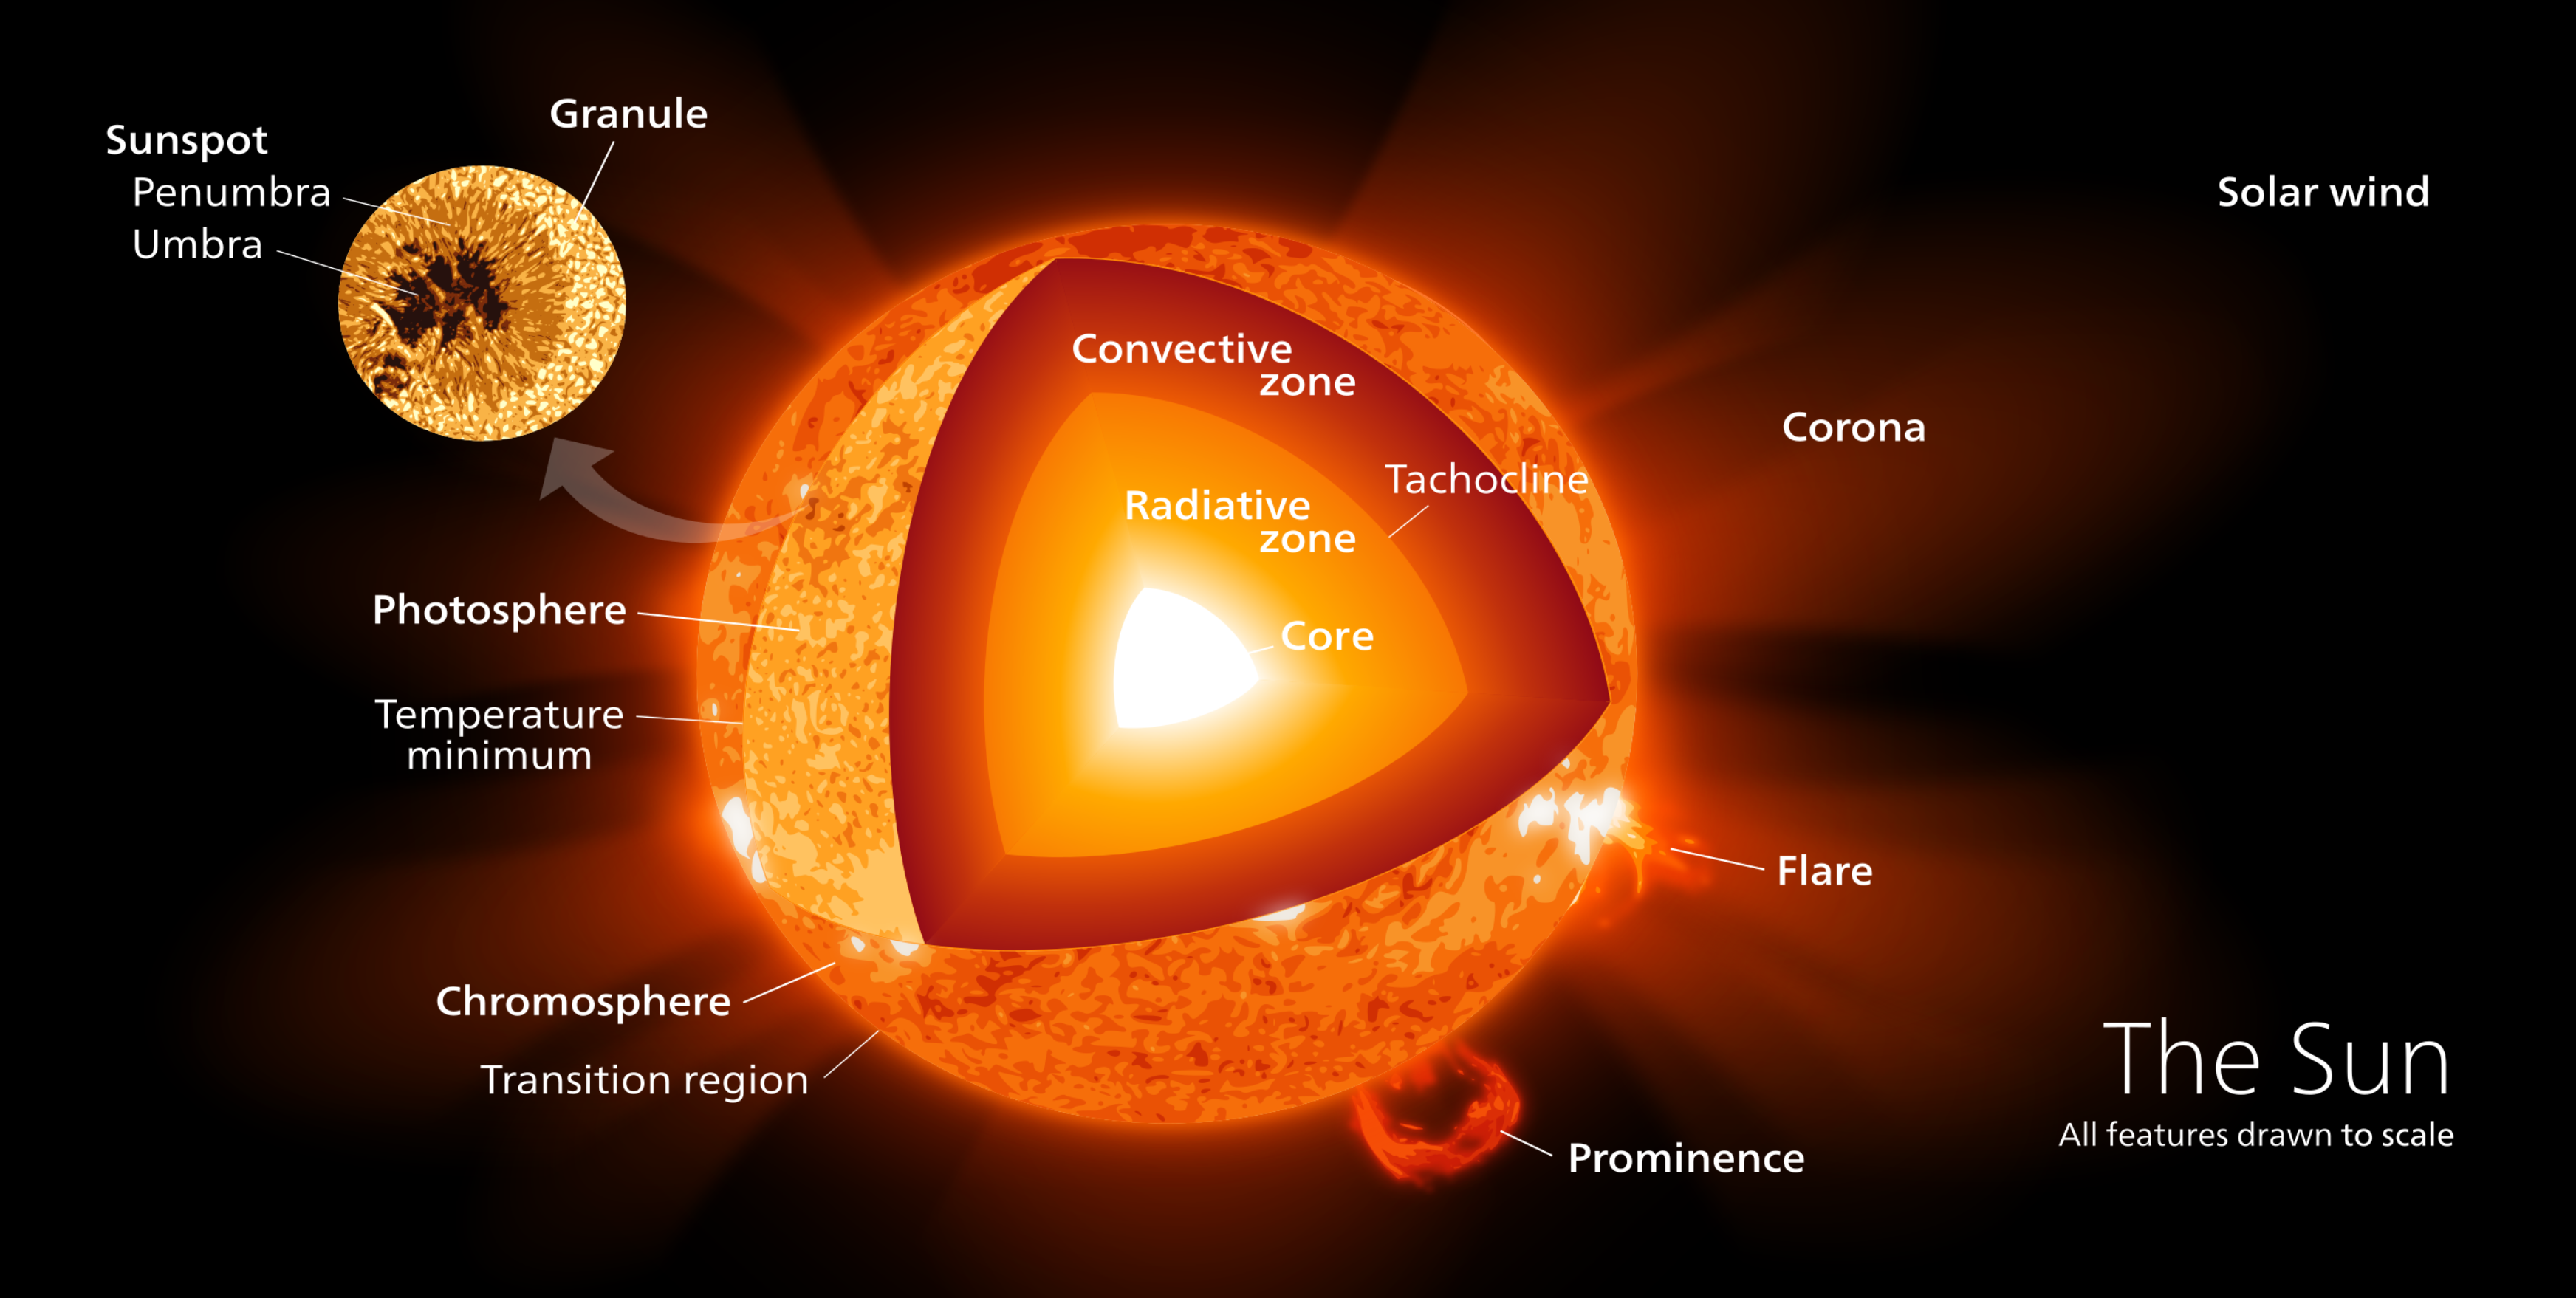
\includegraphics[width=\textwidth]{./pictures/interior.PNG}
    \caption{Visualization of the interior structure of the Sun. \cite{kelvin13}}
    \label{fig:structure}
\end{figure}
In this work we will mainly focus on phenomena related to convection, hence occurring in the convective zone and impacting photosphere.\\
Convection is the transfer of heat from one place to another by the movement of fluids. In particular, regarding the Sun, the temperature at the bottom of the convection zone is 200,000\degree K while at its outermost limit (surface of the Sun) is being cooled by the creation of light and temperature is only about 5700\degree K. This large difference triggers the plasma movement in order to propagate the heat outwards. Note, for instance, in Figure~\ref{fig:convect-cells} the bright regions correspond to hot rising material, whereas the dark lanes are the location where the colder material falls down into the Sun \cite{convect}. Also, as the reader can verify from Figure~\ref{fig:convect-cells} the way convection cells organise on the surface is not regular but rather chaotic and turbulent. \\
\begin{figure}[t]
    \centering
    \begin{subfigure}[b]{0.49\textwidth}
        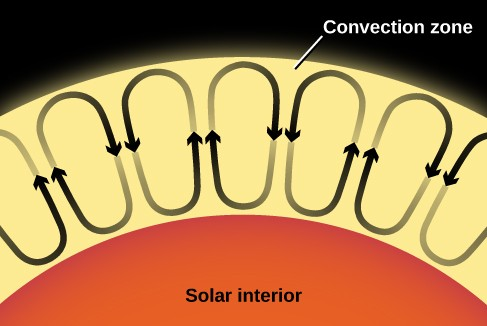
\includegraphics[width=\textwidth]{./pictures/convection}
        \caption{Section view, plasma movement}
        \label{fig:convect}
    \end{subfigure}
    \begin{subfigure}[b]{0.49\textwidth}
        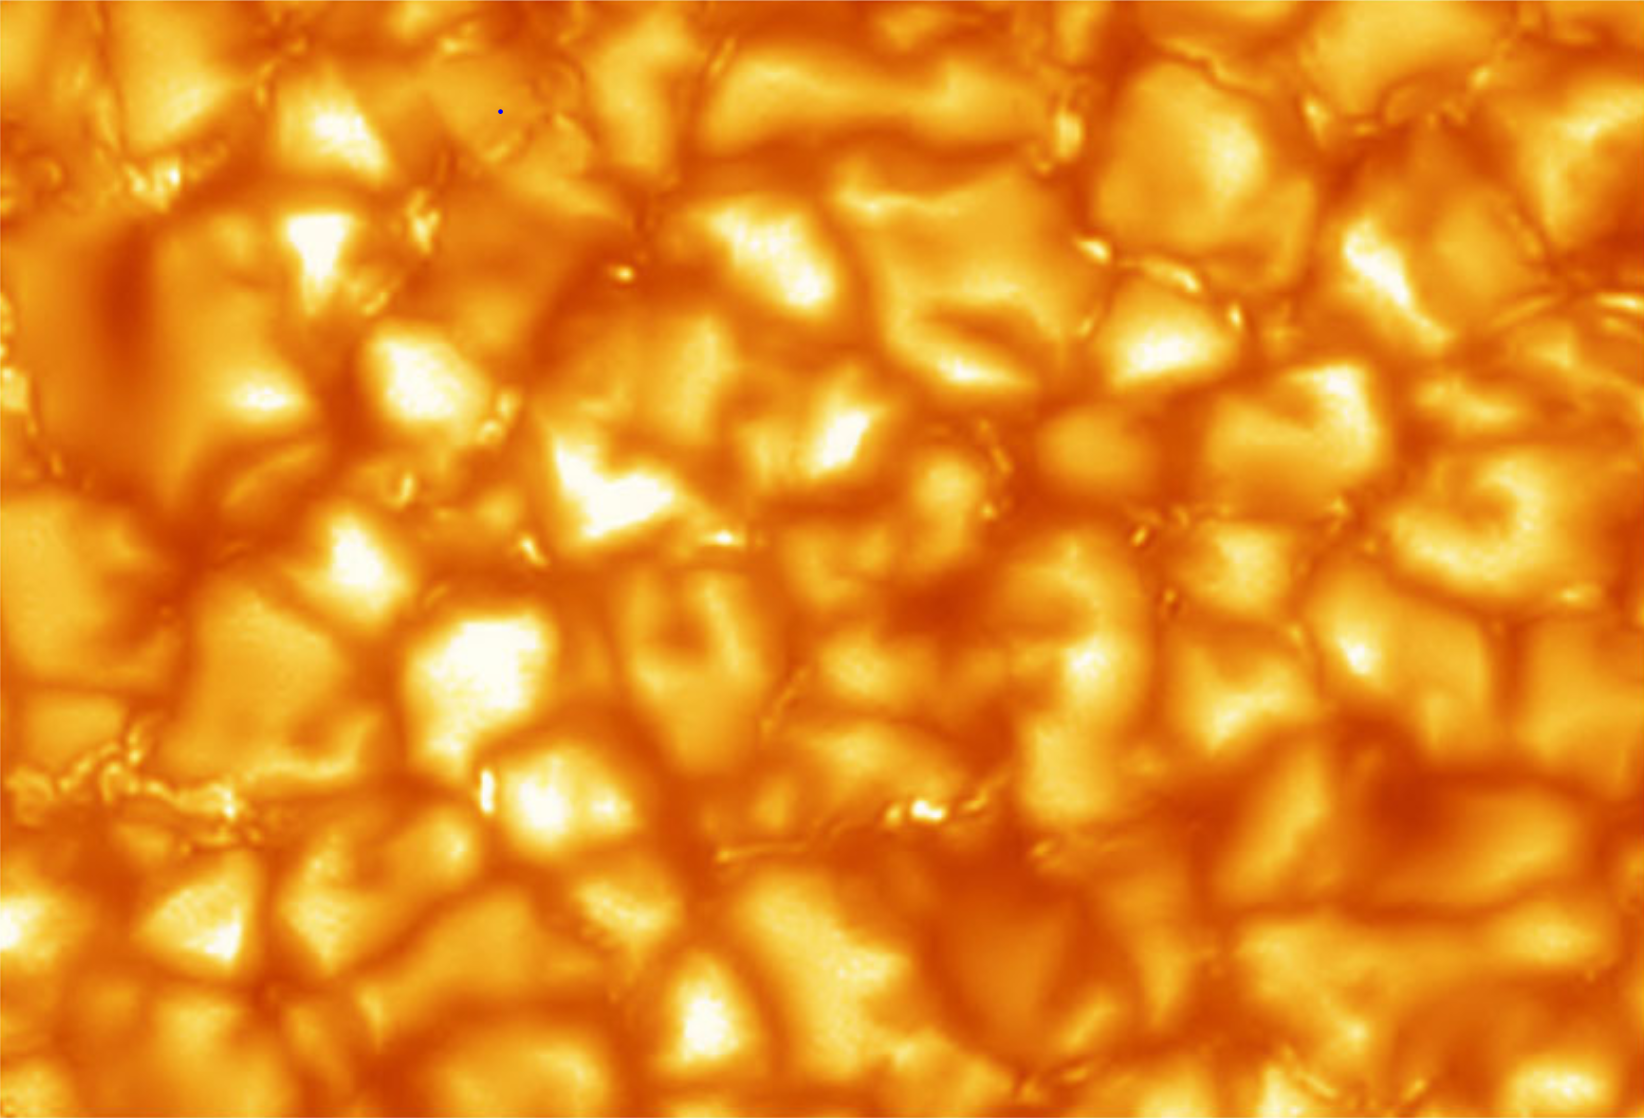
\includegraphics[width=\textwidth]{./pictures/convection-cell}
        \caption{Frontal view, convection cells.}
        \label{fig:convect-cells}
    \end{subfigure}
    \caption{Convection}\label{fig:systemview}
\end{figure}

\begin{figure}[b]
    \centering
    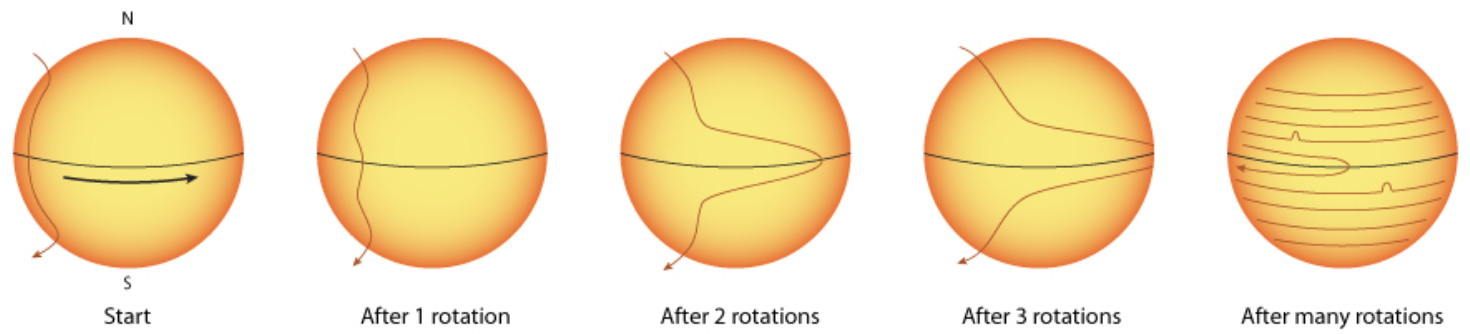
\includegraphics[width=\textwidth]{./pictures/diffrot}
    \caption{Visualization of differential rotation}
    \label{fig:diffrot}
\end{figure}
Another interesting feature of the dynamics of the Sun is its rotation. In fact the sun does not rotate uniformly, since it is not a rigid object (a solid body in which deformation is zero or very small). Our star is composed of gasses in the form of plasma and therefore the relative movement of its inner particles cannot be neglected. This results in a type of motion called differential rotation. It has been observed that the angular velocity of the particles changes in a way that depends on the latitude, in particular it is fastest on the solar equator and decreases as latitude increases \cite{diffrot}. From this notion follows that the rotation period is not constant, it takes 24.47 days at the equator and almost 38 days at the poles \cite{diffrotrev}. Furthermore this behaviour has a critical importance for the understanding of this work for two reasons. First, the features that we studied are located on the photosphere and move with the surface of the Sun, undergoing significant deformation. Second, differential rotation together with convective turbulent motions leads to the generation of electric currents and solar magnetic field. This phenomenon is called solar dynamo and is in some way similar to the dynamo effect that generates the magnetic field of the Earth. Moreover the generated magnetic field has the property that it tends to agglomerate into bundles called magnetic flux tubes. When these tubes become strong enough to locally inhibit convection the heat coming from inside the Sun is not propagated upwards and the temperature of the surface decreases significantly. The local temperature drop makes the affected area look darker than the rest of the disk. These black patches, commonly named \textbf{sunspots}, are fairly easy to observe, even with an amatorial telescope, this is the reason why they have been observed during the last approximately 400 years.
